                                                                                                                                                                                                                                                                                                                                                                                                                                                                                                                                                                                                                                                                                                                                                                                                                                                                                                                                                    %%%%%%%%%%%%%%%%%%%%%%%%%%%%%%%%%%%%%%%%%
% Short Sectioned Assignment LaTeX Template Version 1.0 (5/5/12)
% This template has been downloaded from: http://www.LaTeXTemplates.com
% Original author:  Frits Wenneker (http://www.howtotex.com)
% License: CC BY-NC-SA 3.0 (http://creativecommons.org/licenses/by-nc-sa/3.0/)
%%%%%%%%%%%%%%%%%%%%%%%%%%%%%%%%%%%%%%%%%

%----------------------------------------------------------------------------------------
%	PACKAGES AND OTHER DOCUMENT CONFIGURATIONS
%----------------------------------------------------------------------------------------

\documentclass[paper=a4, fontsize=11pt]{scrartcl} % A4 paper and 11pt font size

% ---- Entrada y salida de texto -----

\usepackage[T1]{fontenc} % Use 8-bit encoding that has 256 glyphs
\usepackage[utf8]{inputenc}
%\usepackage{fourier} % Use the Adobe Utopia font for the document - comment this line to return to the LaTeX default

% ---- Idioma --------

\usepackage[spanish, es-tabla]{babel} % Selecciona el español para palabras introducidas automáticamente, p.ej. "septiembre" en la fecha y especifica que se use la palabra Tabla en vez de Cuadro

% ---- Otros paquetes ----

\usepackage{amsmath,amsfonts,amsthm} % Math packages
%\usepackage{graphics,graphicx, floatrow} %para incluir imágenes y notas en las imágenes
\usepackage{graphics,graphicx, float} %para incluir imágenes y colocarlas

% Para hacer tablas comlejas
%\usepackage{multirow}
%\usepackage{threeparttable}

%\usepackage{sectsty} % Allows customizing section commands
%\allsectionsfont{\centering \normalfont\scshape} % Make all sections centered, the default font and small caps

\usepackage{fancyhdr} % Custom headers and footers
\usepackage{url}
\usepackage{hyperref}
\pagestyle{fancyplain} % Makes all pages in the document conform to the custom headers and footers
\fancyhead{} % No page header - if you want one, create it in the same way as the footers below
\fancyfoot[L]{} % Empty left footer
\fancyfoot[C]{} % Empty center footer
\fancyfoot[R]{\thepage} % Page numbering for right footer
\renewcommand{\headrulewidth}{0pt} % Remove header underlines
\renewcommand{\footrulewidth}{0pt} % Remove footer underlines
\setlength{\headheight}{13.6pt} % Customize the height of the header

\numberwithin{equation}{section} % Number equations within sections (i.e. 1.1, 1.2, 2.1, 2.2 instead of 1, 2, 3, 4)
\numberwithin{figure}{section} % Number figures within sections (i.e. 1.1, 1.2, 2.1, 2.2 instead of 1, 2, 3, 4)
\numberwithin{table}{section} % Number tables within sections (i.e. 1.1, 1.2, 2.1, 2.2 instead of 1, 2, 3, 4)

\setlength\parindent{0pt} % Removes all indentation from paragraphs - comment this line for an assignment with lots of text

\newcommand{\horrule}[1]{\rule{\linewidth}{#1}} % Create horizontal rule command with 1 argument of height

\usepackage{booktabs}




%----------------------------------------------------------------------------------------
%	TÍTULO Y DATOS DEL ALUMNO
%----------------------------------------------------------------------------------------

\title{	
\normalfont \normalsize 
\textsc{{\bf Aprendizaje Automático (2014-2015)} \\ 3º Grado en Ingeniería Informática \\ Universidad de Granada} \\ [25pt] % Your university, school and/or department name(s)
\horrule{0.5pt} \\[0.4cm] % Thin top horizontal rule
\huge Proyecto Final: Airfoil Self-Noise Data Set \\ % The assignment title
\horrule{2pt} \\[0.5cm] % Thick bottom horizontal rule
}

\author{Pedro Antonio Ruiz Cuesta\\Ignacio Martín Requena} % Nombre y apellidos

\date{\normalsize\today} % Incluye la fecha actual

%----------------------------------------------------------------------------------------
% DOCUMENTO
%----------------------------------------------------------------------------------------
\usepackage{graphicx}
\usepackage{listings}
\usepackage[usenames]{color}
\usepackage[urlcolor = blue, hidelinks]{hyperref}

\definecolor{gray97}{gray}{.97}
\definecolor{gray75}{gray}{.75}
\definecolor{gray45}{gray}{.45}
 

\lstset{ frame=Ltb,
     framerule=0pt,
     aboveskip=0.5cm,
     framextopmargin=3pt,
     framexbottommargin=3pt,
     framexleftmargin=0.4cm,
     framesep=0pt,
     rulesep=.4pt,
     backgroundcolor=\color{gray97},
     rulesepcolor=\color{black},
     %
     stringstyle=\ttfamily,
     showstringspaces = false,
     basicstyle=\small\ttfamily,
     commentstyle=\color{gray45},
     keywordstyle=\bfseries,
     %
     numbers=left,
     numbersep=15pt,
     numberstyle=\tiny,
     numberfirstline = false,
     breaklines=true,
   }
 


\lstdefinestyle{consola}
   {basicstyle=\scriptsize\bf\ttfamily,
    backgroundcolor=\color{gray75},
   }
 
\lstdefinestyle{C}
   {language=C,
   }



\begin{document}

\maketitle % Muestra el Título

\newpage %inserta un salto de página

\tableofcontents % para generar el índice de contenidos

\listoffigures

%\listoftables

\newpage



%----------------------------------------------------------------------------------------
%	Cuestion 1
%----------------------------------------------------------------------------------------

\section{Descripción del problema}
Nuestro objetivo durante el desarrollo de todo el proyecto será estudiar la base de datos \href{https://archive.ics.uci.edu/ml/datasets/Airfoil+Self-Noise}{\textcolor{cyan}{\emph{Airfoil Self-Noise Data Set}}} con el fin de poder analizar, predecir y obtener aquellos atributos relevantes para reducir el nivel de presión mediante técnicas de regresion el nivel de presión de sonido escalado (Scaled sound pressure level) medido en decibelios.\\

Para ello utilizaremos diferentes técnicas de regresión con el fin de contrastar y analizar qué modelo se ajusta mejor para resolver el problema.\\

La documentación de todo el proceso de experimentos y pruebas a partir del cual se obtuvo la base de datos que usaremos la podemos encontrar en un documento oficial publicado por la NASA en 1989 con el titulo de \href{http://ntrs.nasa.gov/archive/nasa/casi.ntrs.nasa.gov/19890016302.pdf}{\textcolor{cyan}{\emph{Airfoild Self-Noise and Prediction}}}.


%----------------------------------------------------------------------------------------
% Cuestion 2
%----------------------------------------------------------------------------------------
\section{Descripción de la base de datos usada}

Nuestra base de datos se compone de:
\begin{itemize}

	\item 1503 observaciones

	\item 6 variables:

	\begin{enumerate}
		\item Frecuencia, en Hercios. (\textbf{Frequency})
		\item Ángulo de ataque, en grados. (\textbf{AOA})
		\item Longitud de la cuerda, en metros. (\textbf{CL})
		\item Velocidad de la corriente de aire, en metros por segundo. (\textbf{FSV})
		\item Desplazamiento lateral, en metros. (\textbf{SSDT})
		\item Nivel de presión escalado del sonido, en decibelios. (\textbf{SSPL})
	\end{enumerate}

\end{itemize}

Nosotros utilizaremos una sola respuesta, el nivel de presión escalado del sonido, representado frente a uno o mas del resto de predictores de nuestra base de datos.\\

	
	Todas las variables de la base de datos contienen datos de tipo real menos la frecuencia, que es de tipo entero.
\newpage
%----------------------------------------------------------------------------------------
%	Cuestion 3
%----------------------------------------------------------------------------------------
\section{Resumen del análisis de datos realizado para determinar las técnicas seleccionadas}

En el análisis de nuestra base de datos hemos obtenido los siguientes valores para nuestra \textbf{variable respuesta (SSPL)}:

\subsection{Valores estadísticos descriptivos}
	
	\begin{figure}[H]
\centering
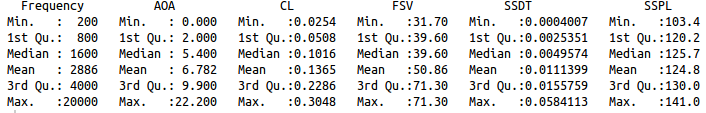
\includegraphics[scale=0.60]{Valores_estadisticos_descriptivos.png}
\caption{Valores estadísticos descriptivos}
\label{ved}
\end{figure}

Como podemos ver en la \textbf{Figura \ref{ved}} el rango de valores de SSPL oscila en esta base de datos entre 103.4 y 141.0 lo que nos lleva a pensar que los valores van a estar muy concentrados (en un rango de apenas 40 decibelios). La mayor cantidad de valores va a estar entorno a 125.7, el valor de la mediana para esta variable. Otro dato a destacar es que la media posee un valor de 124.8, lo cual nos lleva a intuir que, al estar aproximadamente en la mitad entre el valor mínimo y el máximo, es posible que nuestros datos se encuentren dispersos entre estos dos valores, o lo que es lo mismo, no se encuentran muy concentrados cerca del valor mínimo o del máximo.\\


Otro valor estadistico que nos ayuda a obtener información sobre los posibles modelos a ajustar es la \textbf{matriz de correlación}:

\begin{figure}[H]
\centering
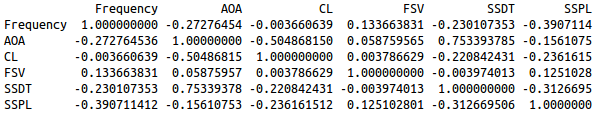
\includegraphics[scale=0.65]{Matriz_de_correlacion.png}
\caption{Matriz de correlación}
\label{mc}
\end{figure}

En la \textbf{Figura \ref{mc}} podemos ver como a priori ningún predictor simple esta muy relacionado con la respuesta , ya que su coeficiente de correlación están lejanos a 1 o -1. Aun así se puede observar que con las variables Frecuency y SSDT quizá se podría obtener resultados relativamente válidos. Como el coeficiente de correlacion nos especifica el grado de relacion entre variables para un modelo lineal simple podemos intuir que el modelo real al que se ajustan los datos probablemente no sea este. Aun así, como tenemos relativamente pocos predictores es viable utilizarlos todos o algunas combinaciones de estos para realizar el ajuste.



	\subsection{Visualizaciónes gráficas}
	
En primer lugar representaremos gráficamente todas las variables con todas para dar un primer vistazo a la relación que existe entre ellas.


	\begin{figure}[H]
\centering
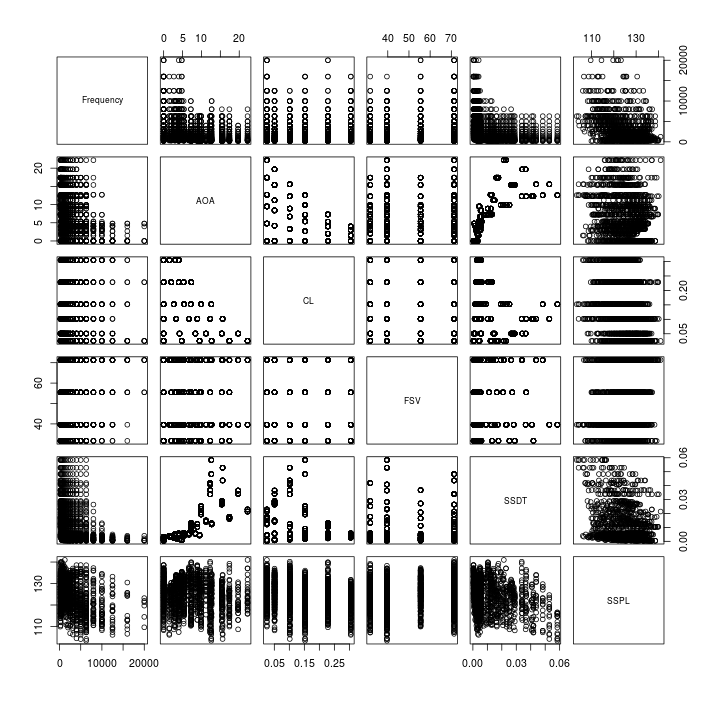
\includegraphics[scale=0.5]{pairs.png}
\caption{Relacion gráfica entre pares de variables}
\label{pairs}
\end{figure}

A simple vista la relación entre nuestra respuesta y los predictores no se observa que no se observa que exista a simple vista, tal y como hemos visto en la \textbf{Figura \ref{ved}}. Fijandonos en el resto de relaciones vemos como entre ADA y SSDT si existe una relación logarítmica, lo que nos puede ayudar a la hora de buscar alguna combinación entre variables\\
	
Todo lo comentado anteriormente sobre la \textbf{Figura \ref{pairs}} se puede ver graficamente en el siguiente \textbf{histograma}:
	
	\begin{figure}[H]
\centering
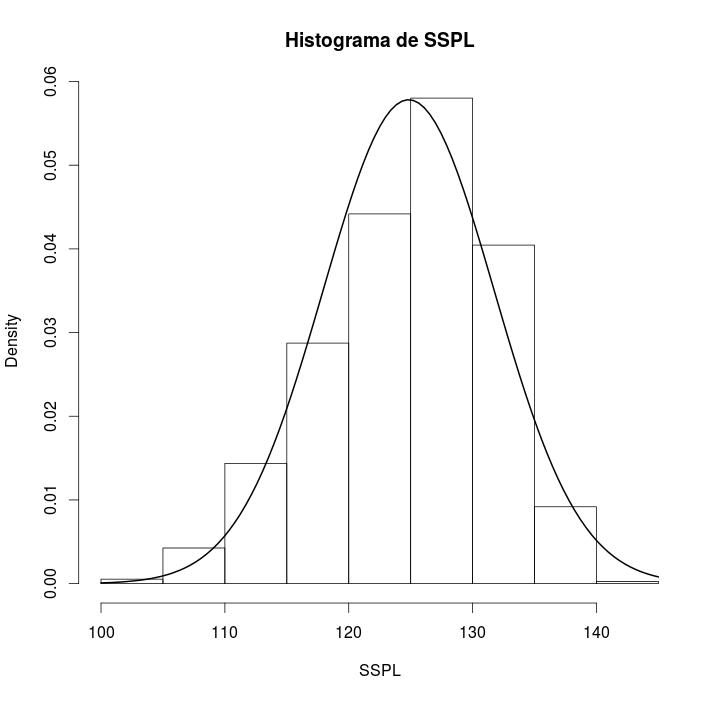
\includegraphics[scale=0.45]{HistogramaSSPL.png}
\caption{Histograma SSPL}
\label{}
\end{figure}

Como se esperaba, el mayor número de observaciones con un valor SSPL cercano a la mediana no lo encontramos justo en el centro si no que se encuentra un poco desplazado, tal y como nos indicaba la mediana teniendo un valor mayor que la media.\\

Otro gráfico que nos puede ayudar a la hora de analizar las variables es el \textbf{diagrama de cajas}:


\begin{figure}[H]
\centering
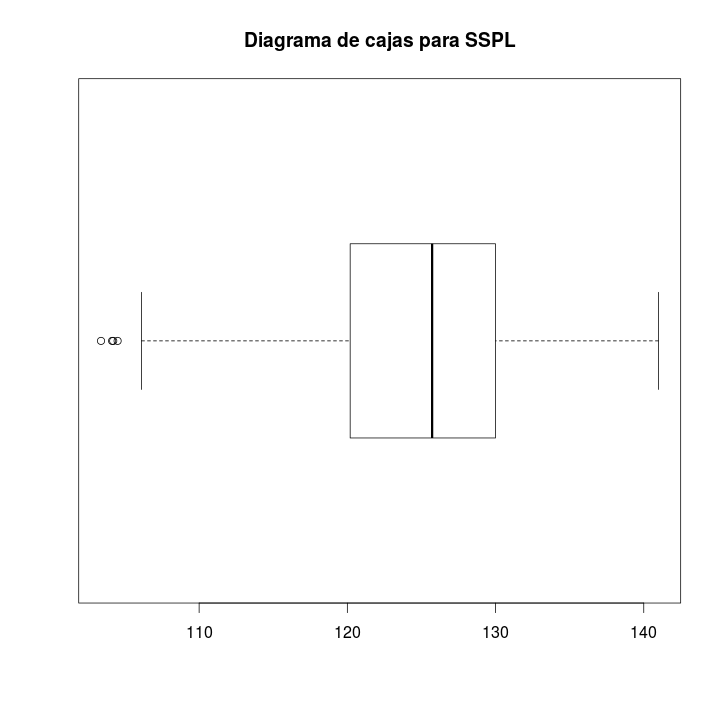
\includegraphics[scale=0.40]{boxplot_SSPL.png}
\caption{Diagrama de cajas SSPL}
\label{}
\end{figure}

En este diagrama observamos que la varianza de los valores menores que la mediana va a ser bastante mayor que los que superan a esta. En concreto, si calculamos la varianza de cada uno de los dos subconjuntos obtenemos que para los valores por debajo de la mediana su varianza es 2,27 veces mayor que los que superan la mediana (22,64 frente a 9,97).



%----------------------------------------------------------------------------------------
%	Cuestion 4
%----------------------------------------------------------------------------------------
\section{Resumen de la metodología llevada a cabo en el ajuste de los modelos empleados}


\subsection{Elección de datos de test y train}

Para la selección de los conjuntos de train y test hemos dividido la base de datos aleatoriamente en dos subconjuntos con el 80\% de las observaciones originales y un 20\% respectivamente.



\subsection{Análisis de de la dependencia entre variables}

Ahora vamos a analizar las variables que nuestra base de datos posee para elegir aquellas que de verdad nos aporten información a la hora de ajustar nuestros modelos, es decir, aquellas variables o combinaciones de variables que hacen nuestro modelo lo mas simple y eficaz posible.\\

En primer lugar representaremos como el coeficiente RSQ va creciendo en función del número de variables seleccionadas para un modelo de regresión, incluyendo las combinaciones de las variables originales:

\begin{figure}[H]
\centering
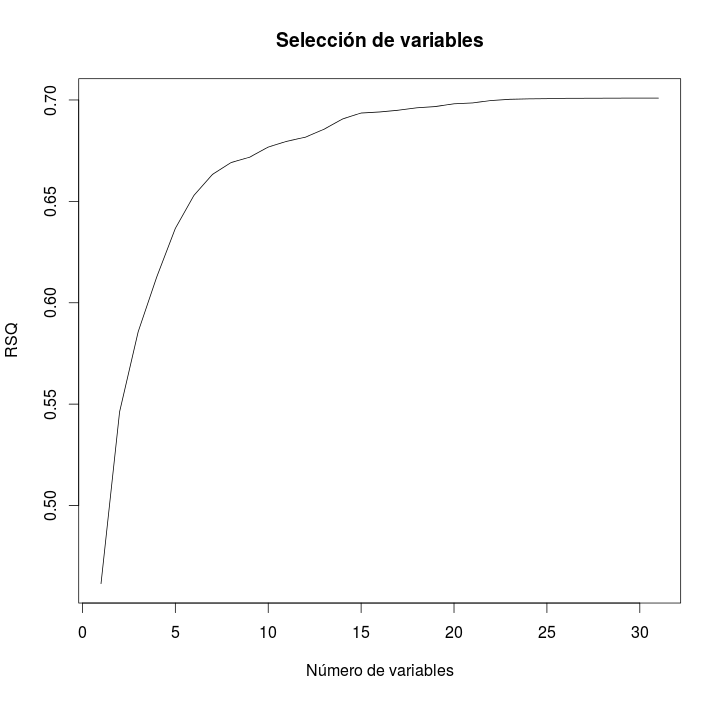
\includegraphics[scale=0.40]{Seleccion_variables.png}
\caption{Numero de variables usadas vs RSQ}
\label{sv}
\end{figure}

Como podemos ver en la \textbf{Figura \ref{sv}}  el coeficiente RSQ para modelos lineales va a ser cercano a 0.7, ya que este valor es el resultado de usar todas las posibles variables incluyendo las combinaciones entre ellas que sería el máximo ajustable que podriamos conseguir, por lo que con nuestros datos a lo sumo conseguiremos que la capacidad del modelo lineal para explicar la variación en la variable respuesta no será superior al 70\%. Para modelos no lineales no podemos predecir a priori cual va a ser el limite máximo de RSQ.\\

Con estos datos deducimos que el incremento de RSQ a partir de usar mas de 20 variables es poco significativo e incluye complejidad a nuestro modelo, por tanto nuestro numero de variables a elegir será este límite.\\

Aplicando el método de selección de busqueda exhaustiva que trata de ajustar un numero definido de modelos con todas las combinaciones de variables predictoras posibles concretaremos las 20 variables a usar.

\begin{table}[h]
\centering

\label{combinaciones}
\begin{tabular}{ccc}
Frequency             & AOA              & FSV                                       \\
Frequency:AOA         & Frequency:CL     & AOA:CL                                    \\
Frequency:FSV         & AOA:FSV          & CL:FSV                                    \\
Frequency:SSDT        & CL:SSDT          & FSV:SSDT                                  \\
Frequency:AOA:CL      & Frequency:CL:FSV & Frequency:AOA:SSDT                        \\
Frequency:CL:SSDT     & AOA:FSV:SSDT     & Frequency:AOA:CL:FSV                      \\
Frequency:AOA:CL:SSDT &                  & \multicolumn{1}{l}{Frequency:CL:FSV:SSDT}
\end{tabular}
\caption{Variables simples y combinadas usadas en el modelo}
\end{table}

\subsection{Elección de técnicas a utilizar}

A raíz de lo expuesto en el apartado anterior y a la vista de los resultados del analisis de datos no podemos intuir la tendencia que van a seguir los datos, ya que en su representación, la variable SSPL no muestra una forma definida. Por tanto se ha elegido una técnica de regresión lineal múltiple debido a su simplicidad y a que es un buen metodo para preveer la dificultad de ajuste de las diferentes técnicas a los datos.\\

Por otro lado se ha optado por aplicar una técnica de Support Vector Machine, ya que al ser versátil aporta una mayor potencia y capacidad de decisión (al poseer diferentes nucleos para cambiar el tipo de ajuste) y por tanto puede que  de mejores resultados.

%----------------------------------------------------------------------------------------
%	Cuestion 5
%----------------------------------------------------------------------------------------
\section{Detalles de la metodología de entrenamiento para cada uno de los modelos empleados}
	
	Para realizar el entrenamiento de las técnicas empleadas se han construido dos subconjuntos de muestras de la base de datos. El primero de ellos, el conjunto de train lo usamos para realizar el ajuste del modelo (conjunto de train) y, una vez ajustado el modelo, con el subconjunto restrante. Como ya se concretó en el apartado 4.2, la distribución de los conjuntos de train y test está determinada en una relación 80-20\% respectivamente.\\
	
	Una vez separada la base de datos en los dos subconjuntos comentados anteriormente, nos centramos en el conjunto de train, con el que obtendremos las relaciones que guardan los predictores con la respuesta. El siguiente paso será elegir, de entre todos los posibles predictores a usar, los que más nos convengan, buscando un compromiso complejidad y ajuste sobre los datos supervisados. Para hacer esta elección de predictores se ha decidido aplicar una técnica de búsqueda exhaustiva ya comentada anteriormente.\\
	
	 Elegido el modelo a ajustar, se procede a realizar dicho ajuste sobre el conjunto de train, este ajuste será el que haga las predicciones a partir de la función ajustada.\\
	
	Después de esto, se realizan las predicciones sobre el conjunto de test. Dichas predicciones, serán las que nos den la bondad del ajuste realizado por la técnica seleccionada.



%----------------------------------------------------------------------------------------
%	Cuestion 7
%----------------------------------------------------------------------------------------
\section{Comparación entre sí de las distintas técnicas usadas con valoración de la idoneidad de cada una para el problema en estudio.}

Para el estudio de la comparación entre los modelos utilizados nos centraremos únicamente en los valores obtenidos para el conjunto de test, que son los realmente relevantes.

\subsection{Comparación gráfica de las predicciones}

Puede ser interesante representar cada una de las predicciones frente a los datos reales para hacernos una idea de que modelo tendrá mayor bondad de ajuste.


\begin{figure}[H]
\centering
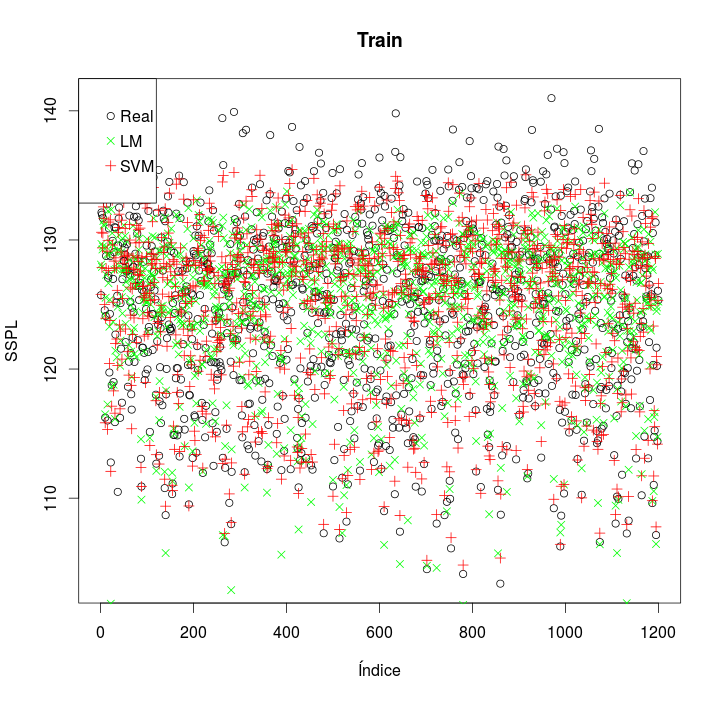
\includegraphics[scale=0.40]{predicciones_train.png}
\caption{Valores reales y valores predichos para train}
\label{}
\end{figure}



\begin{figure}[H]
\centering
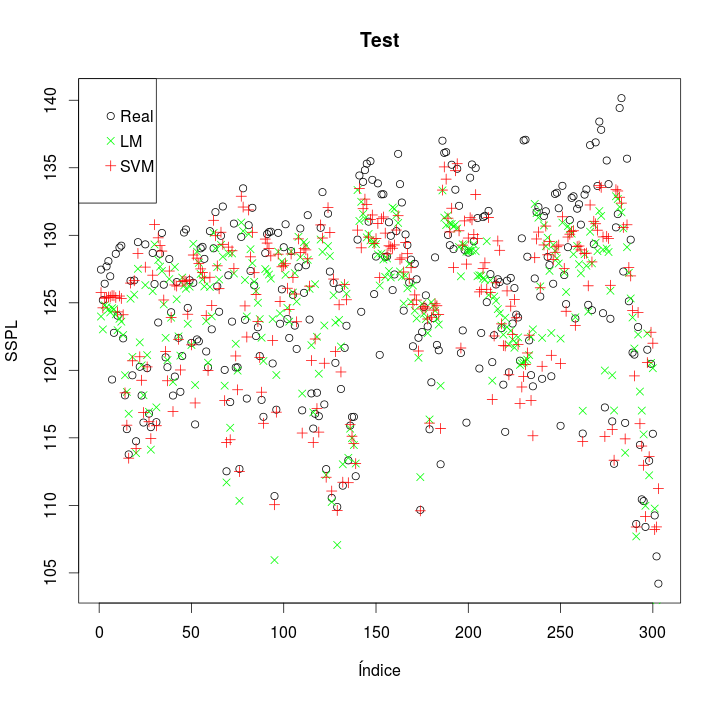
\includegraphics[scale=0.40]{predicciones_test.png}
\caption{Valores reales y valores predichos para test}
\label{}
\end{figure}

A priori vemos que LM tiene algunas predicciones que no se acercan a los datos reales, por ejemplo en zonas en la que los datos están más dispersos. En contraste, SVM no se aleja demasiado de las nubes de puntos reales y, en zonas con alta dispersión su capacidad de predicción es aceptable.\\



Para la comparacion entre las técnicas de ajuste se han obtenido los siguientes valores estadísticos:

\begin{table}[H]
\label{vetrain}
\begin{center}\begin{tabular}{|c|c|c|c|}
\hline
	 & \textbf{RSQ} & \textbf{MSE} & \textbf{SD}\\
\hline
	\textbf{LM} & 0.7 & 14.35 & 5.76\\
\hline
	\textbf{SVM} & 0.81 & 7.69 & 6.21\\
\hline
\end{tabular}\end{center}\centering
\caption{Comparación de bondad de ajuste para train}
\end{table}

\begin{table}[H]
\label{vetest} 
\begin{center}\begin{tabular}{|c|c|c|c|}
\hline
	 & \textbf{RSQ} & \textbf{MSE} & \textbf{SD}\\
\hline
	\textbf{LM} & 0.65 & 14.68 & 5.57\\
\hline
	\textbf{SVM} & 0.75 & 9.66 & 5.99\\
\hline
\end{tabular}\end{center}\centering
\caption{Comparación de bondad de ajuste para test}
\end{table}

\subsection{$R^{2}$}

	Este valor estadístico representa el tanto por ciento de la varianza de los datos que el modelo es capaz de explicar. \\
	
	Al principio comentamos que un modelo lineal no podia tener un valor de $R^{2}$ superior a 0.7, en cambio vemos como SVM supera tal valor. Esto es debido a que se ha utilizado un nucleo radial para el entrenamiento del ajuste. Se hicieron algunas pruebas con otros núcleos como el polinomial, sigmoidal y lineal, pero los resultados obtenidos no fueron superiores al los del uso de un núcleo radial.\\
	
	Basandonos en los valores obtenidos para cada modelo podemos observar como SVM es capaz de explicar los datos introducidos un 15,38\% más que LM.

\subsection{Error medio cuadrático}

	Es un valor estadístico que mide el error en la estimación de un modelo determinado, es decir, es un forma de evaluar la diferencia entre un estimador y el valor real de la cantidad que se quiere calcular. El MSE mide el promedio del cuadrado del error, siendo el error el valor en la que el estimador difiere de la cantidad a ser estimada.\\
	
	Como se puede observar en la \textbf{Tabla 6.2}, el valor de este estadístico es menor en SVM que en LM, y por tanto el error que se comete en las predicciones de SVM será menor que en las de LM.

\subsection{Desviación típica}

	La desviación típica es la ``distancia'' entre la media de un conjunto de datos y el valor de cada uno de los datos. Este valor puede sernos útil si comparamos las desviaciones típicas entre las predicciones de cada ajuste y la desviación típica de que realmente tienen los datos (nuestro conjunto de test).\\	
	
	Como la desviación típica real del conjunto de test es de 6.91, cuanto mas cercano esté el valor de la desviación estándar de una desviación más cerca estaremos de realizar unas predicciones acordes con la realidad. En nuestro caso, como podemos ver en la \textbf{Tabla 6.1}, SVM se acerca más al valor real de la desviación típica que LM y, por tanto, tendrá una mayor capacidad de predicción.



%----------------------------------------------------------------------------------------
%	Cuestion 8
%----------------------------------------------------------------------------------------
\section{Valoración final de los resultados obtenidos.}

Cuando se comenzó a hacer el análisis exploratorio en los primeros pasos se pensaba que no se podría sacar una predicción decente, ya que los datos de la variable respuesta estaban muy repartidos y la dependencia entre variables no era significativa a simple vista (\textbf{Figura \ref{pairs}}).\\

Realizando un análisis de dependencia entre variables y combinandolas entre ellas se consiguió obtener un modelo que aportaba más información y, por tanto, mejores resultados.\\

Con las técnicas seleccionadas la bondad de ajuste conseguida se puede considerar aceptable en relacion a lo esperado. Los resultados obtenidos en las predicciones de las dos técnicas de ajuste aplicadas (LM y SVM) así como los valores estadísticos obtenidos ($R^{2}$, MSE y SD) muestran como la diferencia entre las predicciones y los valores reales es asumible.

%----------------------------------------------------------------------------------------
%	Cuestion 4
%----------------------------------------------------------------------------------------
\section{Conclusiones.}

Al ser un problema con un alto grado de incertidumbre y de interacción entre los atributos, el error asociado a la medición de los valores de nuestro modelo será alto y, por tanto,  \\

Como el objetivo final de este estudio es intentar predecir el nivel de presion de sonido con el fin de, a partir de los modelos de predicción obtenidos, poder reducirlo, se llega a la conclusión de que si se mejoran los valores de frecuencia (predictor más influyente), ángulo de ataque y la velocidad de la corriente de aire (variables más frecuentes en nuestro modelo, especificadas en la \textbf{Tabla \ref{combinaciones}}) el nivel de presión escalado del sonido mejorará también.



\end{document}